\documentclass[12pt]{article}

\usepackage{amsmath}
\usepackage{amsfonts}
\usepackage{graphicx}
\usepackage[subrefformat=parens]{subcaption}
\usepackage{booktabs}
\usepackage{multirow}
\usepackage{rotating}
\usepackage[table]{xcolor}
\usepackage{url}
\usepackage{hyperref}

\title{Classifying perceived object count from fMRI time series}
\author{Andrew Floren}
\date{}

\bibliographystyle{ieeetr}

\begin{document}

\maketitle{}

\section{Aims}
Traditionally, fMRI has been used to study the spatial and temporal correlation of metabolic activity in the brain with various external activities or tasks.
A recent trend in the field has seen machine learning applied to fMRI data in an attempt to blindly predict the external activity or task from the pattern of activation \cite{Haxby2001,Mitchell2003,Haynes2006}.
In this way, researchers hope to uncover more complex relationships between the patterns of activation and the external activity.
Thus far, researchers have been successful in differentiating the patterns of activation that result from subjects viewing broad categories of objects.
For example, the researchers in \cite{Haxby2001} were able to differentiate the pattern of activation created by a subject viewing an image of a face from the pattern created by a subject viewing a house and a variety of other object categories.
Using these predictive methods as tools, other researchers have assembled a number of insightful cognitive and behavioral studies \cite{Lewis-Peacock2012,Davatzikos2005}.
However, these studies are limited to the dimensions that can be resolved by the current predictive methods; i.e., we can resolve the difference between a subject viewing a face and a place, but not between a subject viewing two different faces.
Our first goal is to introduce and evaluate a new resolvable dimension, specifically the perceived count of broad object categories (e.g., the number of faces that a subject perceives in a stimulus).
Our second goal is to develop better predictive methods for increasing the resolution along resolvable dimensions in general.

The current lack of resolvable dimensions is due in large part to the novelty of the approach.
There is a wealth of information regarding correlation analyses between functional activation and all manner of tasks, but so far the number of tasks that predictive methods have been applied to is limited.
The resolution along dimensions is limited in part by measurement noise; this includes noise introduced by the scanner as well as cognitive processes.
However, the resolution is also limited by the quality of the predictive methods utilized.
Thus far, only relatively simple machine learning algorithms have been employed due to the necessary cross-disciplinary collaboration required for implementing and properly analyzing more complex machine learning techniques.

Our own preliminary results suggest that it should be possible to predict the number of objects a subject is viewing and this is where we will be focusing the initial stages of our research.
We will evaluate the precision and accuracy with which this dimension can be predicted.
Being able to classify what the subject is viewing and how many will allow researchers to develop new cognitive and behavioral studies. 
Additionally, we will experiment with more state of the art machine learning algorithms in order to improve the resolution with which we can measure this dimension and dimensions in general.

\section{Background}
Our experiment will employ both 

\subsection{Functional MRI}
Functional magnetic resonance imaging (fMRI) is an application of MRI at speeds that allow for the imaging of fast changing physiological events instead of more static anatomical information.
Most commonly, fMRI is employed to measure localized functional activation in the brain.
This measurement is made possible by the fact that deoxygenated hemoglobin in the blood is a naturally occurring contrast agent for MRI.
The fluctuation in the measured MRI signal induced by the relative local concentration of oxygenated and deoxygenated hemoglobin is known as the blood oxygenation level-dependent (BOLD) contrast \cite{Ogawa1990}.
In turn, BOLD contrast can be used to localize activation in the brain thanks to the neural hemodynamic response.
Neural activity requires increased metabolic activity including increased oxygen uptake (i.e., CMR02).
To compensate for this increased uptake, the brain must in turn supply more oxygen to the activated regions.
Through vascular regulation, the brain is able to direct increased blood flow and thus more oxygenated blood to highly localized areas of the brain \cite{Buxton2004}.
In this way, the BOLD contrast is coupled with local neural activity.

However, the contrast induced by neural activity is extremely small, on the order 1\%.
Worse still, the noise variance of fMRI data is also on the order of 1\%.
Therefore, fMRI experiments are designed to maximize detection power when the signal to noise ratio (SNR) is approximately unity.
The two most common experiment paradigms are blocked and event related.
In blocked experiment designs, the subject is presented with a stimulus or task for a fixed time period after which they are presented with a second stimulus or task for the same time period.
The two blocks alternate for the duration of the scan.
In event related design, events or stimuli appear at random intervals for relatively brief durations.
The simple blocked design has greater detection power but the event related design is more flexible in terms of what can be measured \cite{Dale1997,Liu2001}.
Once the data has been collected, statistical anlysis is used to calculate the confidence with which conclusions can be drawn from the data.
A wide range of tools has been developed for this purpose \cite{Bandettini1993}, from coherence analyses to generalized linear model approaches \cite{Worsley1995,Beckmann2003}.

\subsection{Machine Learning}
Machine learning is a broad term for algorithms that are able to learn or improve their performance on large datasets.
We will specifically be dealing with supervised classification algorithms which learn from a large dataset of pre-classified or labeled examples how to classify new data points.
Many machine learning algorithms draw intuition from our understanding of the human brain, most notably the perceptron and neural network \cite{Hecht-nielsen1989,Jain1996}.
A general neural network is a very powerful tool, however efficient methods for training such a machine have proven elusive.
On the other hand, more constrained feed-forward neural networks have found much success using relatively simple back-propagation training techniques.
One of the most popular machine learning algorithms is the support vector machine (SVM).
Although it is not generally considered a neural network algorithm, the SVM was called a support-vector network by its original author and much intuition was drawn from existing neural network literature \cite{Cortes1995}.
For a simple two-class problem, the SVM tries to find a single hyperplane which maximally separates all data points in the labeled dataset.
This hyerplane is then used to classify new data points.
In the case that a single separating hyperplane does not exist, the algorithm will still converge to a highly discriminative hyperplane.
Furthermore, the SVM can be modified to support $N$-class problems by solving for $N-1$ hyperplanes which separate all of the classes.
The authors of \cite{Burges1998} have written an excellent tutorial article covering the application of the SVM to classification and pattern recognition

\subsection{Machine Learning applied to fMRI}
The abundance of data and the relatively high dimensionality would seem to make machine learning a natural fit for application to fMRI data.
The authors of \cite{Haxby2001} were the first to utilize machine learning methods in their analysis.
In their experiment, they tested the discriminability of the perception of various object categories including faces, houses, and other manmade objects.
Interestingly, they showed that the patterns of activation were easily classified by machine learning algorithms but that those patterns were also highly overlapping.
This distributed and overlapping nature of many processes in the brain can confound more classical statistical analysis methods.
The authors of \cite{Mitchell2003} and \cite{Haynes2006} helped to expand this concept and introduced methods for producing maps of task correlated activity using sensitivity analysis.

The majority of the existing literature in this area focuses on the discriminability of the perception of broad object categories discovered in \cite{Haxby2001}.
Unfortunately, this has limited the acceptance of machine learning as a broader analytical tool in fMRI.
Some very promising experiments such as \cite{Lewis-Peacock2012} have been developed to properly utilize these algorithms but they all adhere firmly to the well-documented and well-analyzed object category discrimination stimulus.
By documenting and analyzing new and interesting stimuli that can be measured using machine learning algorithms we will open the door for exciting new opportunities in cognitive and behavioral neuroscience.

Another reason that experiments utilizing machine learning as an analysis method have by and large only used the object category discrimination stimulus is likely due to the fact that the stimulus generates very easily recognizable patterns.
Most machine learning algorithms will have no problem attaining near perfect performance on a well collected dataset using this stimulus.
This instills a very high level of confidence in conclusions drawn from the results.
By developing improved machine learning techniques specifically for fMRI data we will be able to improve researchers' confidence in conclusions drawn from a wider variety of stimulus designs.

\subsection{Face Perception and Counting Tasks}
Object recognition and specifically face recognition areas of the brain have been studied for some time \cite{McCarthy1997}. 
It is for this reason that the authors of \cite{Haxby2001} likely chose it for their first foray into machine learning techniques. 
On the other hand, counting or the perception of number is much less studied in the fMRI domain.
Many stimuli use counting as part of the task a subject performs while viewing a stimulus \cite{Bush1998,Mostofsky2003}.
However, these experiments are generally not concerned with the neural representation of the count and it would be more of a confound in their results than anything else.
In other experiments, researchers are interested in identifying the part of the brain associated with arithmetic computation \cite{Rickard2000,Eliez2001}, but again these experiments are not concerned with specific counts or values of the computation being performed.
It is likely that the neural representation of count is both highly overlapping and highly distributed depending on the type of counting being performed and thus classical statistical analysis approaches would have a difficult time discriminating them. 
This overlapping and distributed nature makes perceived count a perfect target for a machine learning approach.

\section{Preliminary/Expected Results}
We have preliminary data indicating that it should be possible to predict the number of faces that a subject is viewing.
In another study we collected fMRI time series data while the subject viewed a complex virtual world stimulus.
The stimulus takes place in a virtual town where the subject alternates between moving through the virtual town and viewing animated characters.
An example frame from the stimulus appears in figure \ref{fig:preliminary-data-frame}.
\begin{figure}
\centering
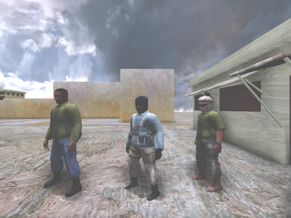
\includegraphics[width=0.5\textwidth]{figures/preliminary-data-frame}
\caption{An example frame from the stimulus used in our preliminary experiment.
The number of characters in the scene were successfully predicted from the fMRI time series data despite the complex scene and camera motion.}
\label{fig:preliminary-data-frame}
\end{figure}
Using both feed forward neural networks and a linear SVM we were able to successfully predict the number of characters that a subject was viewing.
The accuracy results for both the neural network and linear SVM are summarized as confusion matrices in figure \ref{fig:preliminary-data-confusion}.
\begin{figure}
\centering
\begin{subfigure}{\textwidth}
\centering

\begin{tabular}{*{8}{c}}
& & \multicolumn{6}{c}{predicted count} \\
& & 1 & 2 & 3 & 4 & 5 & 6 \\
\multirow{6}{*}{\begin{sideways}actual count\end{sideways}}
& 1 & \cellcolor[rgb]{0.246268656716,0.753731343284,0.0}404 & \cellcolor[rgb]{0.942164179104,0.0578358208955,0.0}31 & \cellcolor[rgb]{0.917910447761,0.0820895522388,0.0}44 & \cellcolor[rgb]{0.966417910448,0.0335820895522,0.0}18 & \cellcolor[rgb]{0.973880597015,0.0261194029851,0.0}14 & \cellcolor[rgb]{0.953358208955,0.0466417910448,0.0}25 \\
& 2 & \cellcolor[rgb]{0.937153419593,0.0628465804067,0.0}34 & \cellcolor[rgb]{0.475046210721,0.524953789279,0.0}284 & \cellcolor[rgb]{0.913123844732,0.086876155268,0.0}47 & \cellcolor[rgb]{0.866913123845,0.133086876155,0.0}72 & \cellcolor[rgb]{0.946395563771,0.0536044362292,0.0}29 & \cellcolor[rgb]{0.861367837338,0.138632162662,0.0}75 \\
& 3 & \cellcolor[rgb]{0.92700729927,0.0729927007299,0.0}40 & \cellcolor[rgb]{0.905109489051,0.0948905109489,0.0}52 & \cellcolor[rgb]{0.467153284672,0.532846715328,0.0}292 & \cellcolor[rgb]{0.802919708029,0.197080291971,0.0}108 & \cellcolor[rgb]{0.930656934307,0.0693430656934,0.0}38 & \cellcolor[rgb]{0.967153284672,0.0328467153285,0.0}18 \\
& 4 & \cellcolor[rgb]{0.955555555556,0.0444444444444,0.0}24 & \cellcolor[rgb]{0.885185185185,0.114814814815,0.0}62 & \cellcolor[rgb]{0.790740740741,0.209259259259,0.0}113 & \cellcolor[rgb]{0.633333333333,0.366666666667,0.0}198 & \cellcolor[rgb]{0.833333333333,0.166666666667,0.0}90 & \cellcolor[rgb]{0.901851851852,0.0981481481481,0.0}53 \\
& 5 & \cellcolor[rgb]{0.970802919708,0.029197080292,0.0}16 & \cellcolor[rgb]{0.92700729927,0.0729927007299,0.0}40 & \cellcolor[rgb]{0.899635036496,0.100364963504,0.0}55 & \cellcolor[rgb]{0.81204379562,0.18795620438,0.0}103 & \cellcolor[rgb]{0.496350364964,0.503649635036,0.0}276 & \cellcolor[rgb]{0.894160583942,0.105839416058,0.0}58 \\
& 6 & \cellcolor[rgb]{0.893442622951,0.106557377049,0.0}52 & \cellcolor[rgb]{0.801229508197,0.198770491803,0.0}97 & \cellcolor[rgb]{0.963114754098,0.0368852459016,0.0}18 & \cellcolor[rgb]{0.885245901639,0.114754098361,0.0}56 & \cellcolor[rgb]{0.883196721311,0.116803278689,0.0}57 & \cellcolor[rgb]{0.573770491803,0.426229508197,0.0}208 \\
\end{tabular}

\caption{}
\label{fig:svm-confusion}
\end{subfigure}
\begin{subfigure}{\textwidth}
\centering

\begin{tabular}{*{8}{c}}
& & \multicolumn{6}{c}{predicted count} \\
& & 1 & 2 & 3 & 4 & 5 & 6 \\
\multirow{6}{*}{\begin{sideways}actual count\end{sideways}}
& 1 & \cellcolor[rgb]{0.376736111111,0.623263888889,0.0}359 & \cellcolor[rgb]{0.925347222222,0.0746527777778,0.0}43 & \cellcolor[rgb]{0.875,0.125,0.0}72 & \cellcolor[rgb]{0.921875,0.078125,0.0}45 & \cellcolor[rgb]{0.987847222222,0.0121527777778,0.0}7 & \cellcolor[rgb]{0.913194444444,0.0868055555556,0.0}50 \\
& 2 & \cellcolor[rgb]{0.899305555556,0.100694444444,0.0}58 & \cellcolor[rgb]{0.541666666667,0.458333333333,0.0}264 & \cellcolor[rgb]{0.899305555556,0.100694444444,0.0}58 & \cellcolor[rgb]{0.873263888889,0.126736111111,0.0}73 & \cellcolor[rgb]{0.946180555556,0.0538194444444,0.0}31 & \cellcolor[rgb]{0.840277777778,0.159722222222,0.0}92 \\
& 3 & \cellcolor[rgb]{0.930555555556,0.0694444444444,0.0}40 & \cellcolor[rgb]{0.913194444444,0.0868055555556,0.0}50 & \cellcolor[rgb]{0.560763888889,0.439236111111,0.0}253 & \cellcolor[rgb]{0.769097222222,0.230902777778,0.0}133 & \cellcolor[rgb]{0.9375,0.0625,0.0}36 & \cellcolor[rgb]{0.888888888889,0.111111111111,0.0}64 \\
& 4 & \cellcolor[rgb]{0.947916666667,0.0520833333333,0.0}30 & \cellcolor[rgb]{0.894097222222,0.105902777778,0.0}61 & \cellcolor[rgb]{0.791666666667,0.208333333333,0.0}120 & \cellcolor[rgb]{0.664930555556,0.335069444444,0.0}193 & \cellcolor[rgb]{0.859375,0.140625,0.0}81 & \cellcolor[rgb]{0.842013888889,0.157986111111,0.0}91 \\
& 5 & \cellcolor[rgb]{0.949652777778,0.0503472222222,0.0}29 & \cellcolor[rgb]{0.921875,0.078125,0.0}45 & \cellcolor[rgb]{0.899305555556,0.100694444444,0.0}58 & \cellcolor[rgb]{0.815972222222,0.184027777778,0.0}106 & \cellcolor[rgb]{0.559027777778,0.440972222222,0.0}254 & \cellcolor[rgb]{0.854166666667,0.145833333333,0.0}84 \\
& 6 & \cellcolor[rgb]{0.904513888889,0.0954861111111,0.0}55 & \cellcolor[rgb]{0.869791666667,0.130208333333,0.0}75 & \cellcolor[rgb]{0.901041666667,0.0989583333333,0.0}57 & \cellcolor[rgb]{0.850694444444,0.149305555556,0.0}86 & \cellcolor[rgb]{0.888888888889,0.111111111111,0.0}64 & \cellcolor[rgb]{0.585069444444,0.414930555556,0.0}239 \\
\end{tabular}

\caption{}
\label{fig:nn-confusion}
\end{subfigure}
\caption{The confusion matrices for the \subref{fig:svm-confusion} linear SVM and the \subref{fig:nn-confusion} feed-forward neural network trained on our preliminary data.
Each cell contains the number of frames that contained a specific character count, as indicated by the row, that were classified as some other character count, as indicated by the column.
Therefore, the cells along the diagonal indicate correctly classified frames.}
\label{fig:preliminary-data-confusion}
\end{figure}
Each cell in a confusion matrix contains the number of examples from one class, indicated by the row, that were classified as another class, indicated by the column.
Therefore, the cells along the diagonal indicate correctly classified examples.
The color of the cell indicates the percent of examples that fall in that cell out of all examples in the row.
Completely red indicates zero percent while completely green indicates one-hundred percent.
If the classifiers were guessing randomly then every cell would be the same color.
On average, the classifiers are able to correctly classify the examples over fifty percent of the time.

However, the stimulus was very complex which makes it difficult to tease apart precisely what dimension the classification algorithms were measuring.
A sensitivity analysis indicated that the majority of useful information for training the neural network is contained primarily in the occipital lobe along both the ventral and dorsal visual streams.
This sensitivity analysis is presented in figure \ref{fig:preliminary-data-sensitivity}.
\begin{figure}
\centering
\begin{subfigure}{0.4\textwidth}
\centering
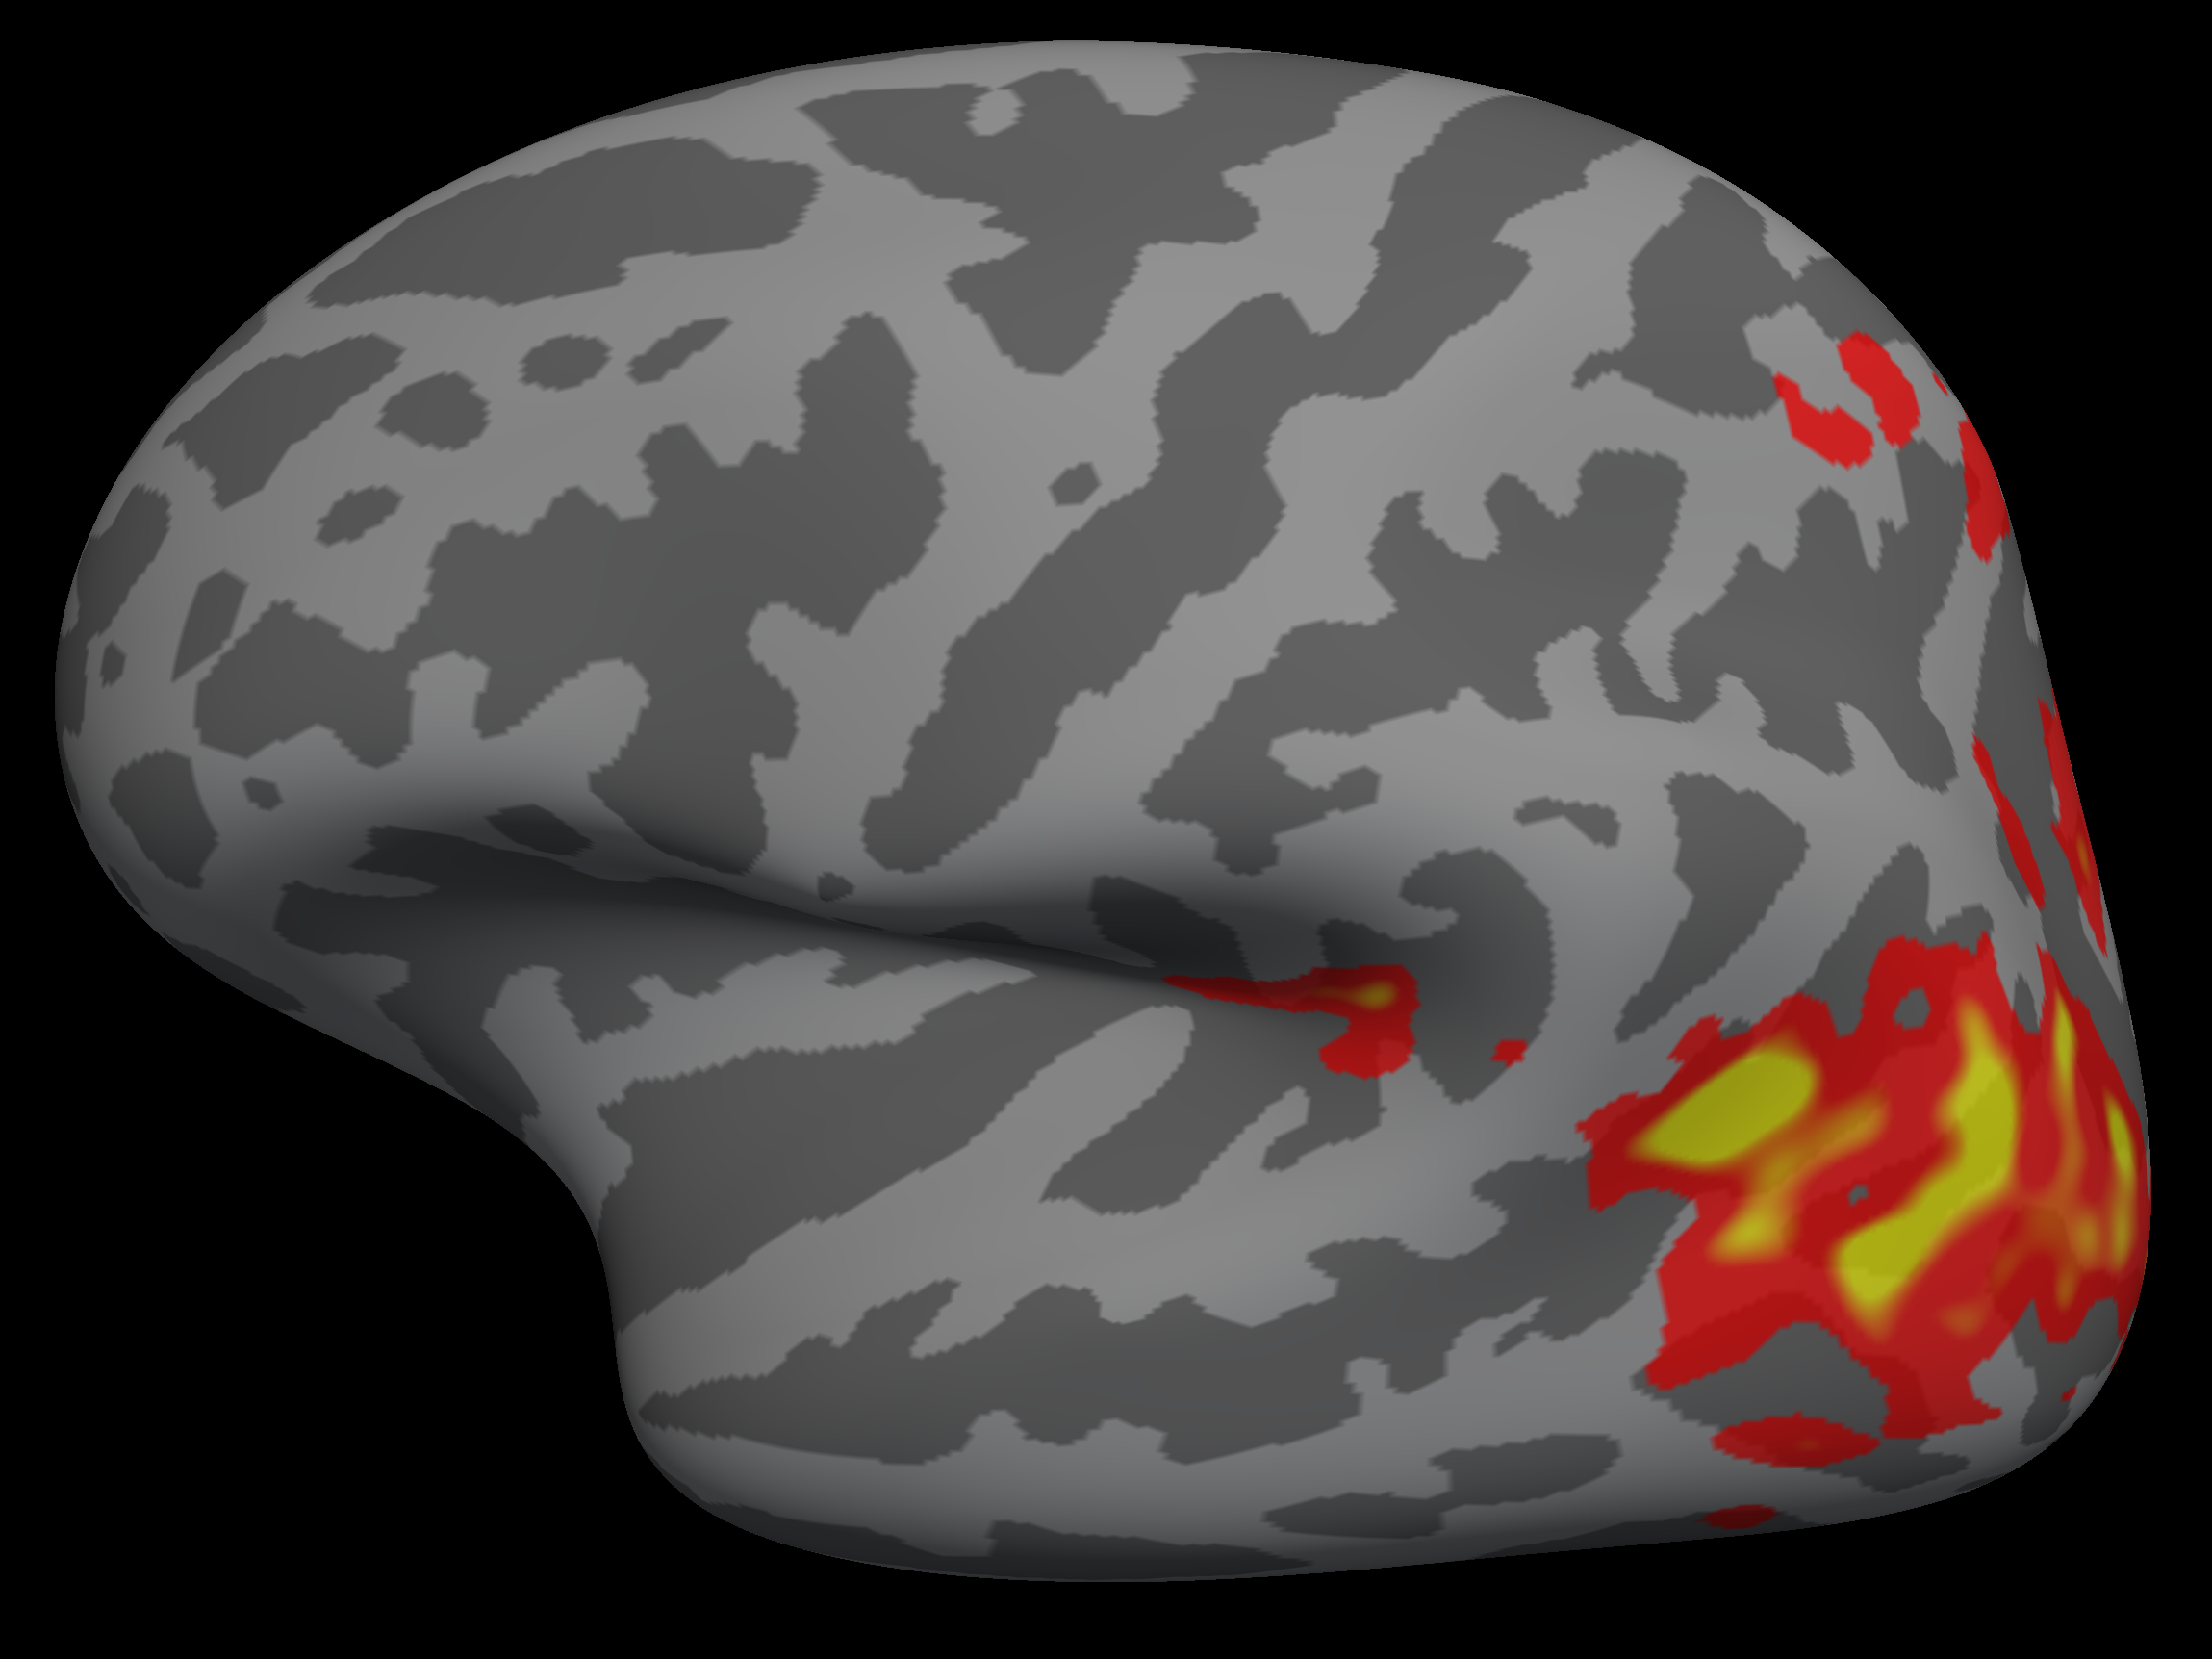
\includegraphics[width=\textwidth]{figures/lh-lateral-smax-average}
\caption{}
\label{fig:lh-lateral-smax-average}
\end{subfigure}
\begin{subfigure}{0.4\textwidth}
\centering
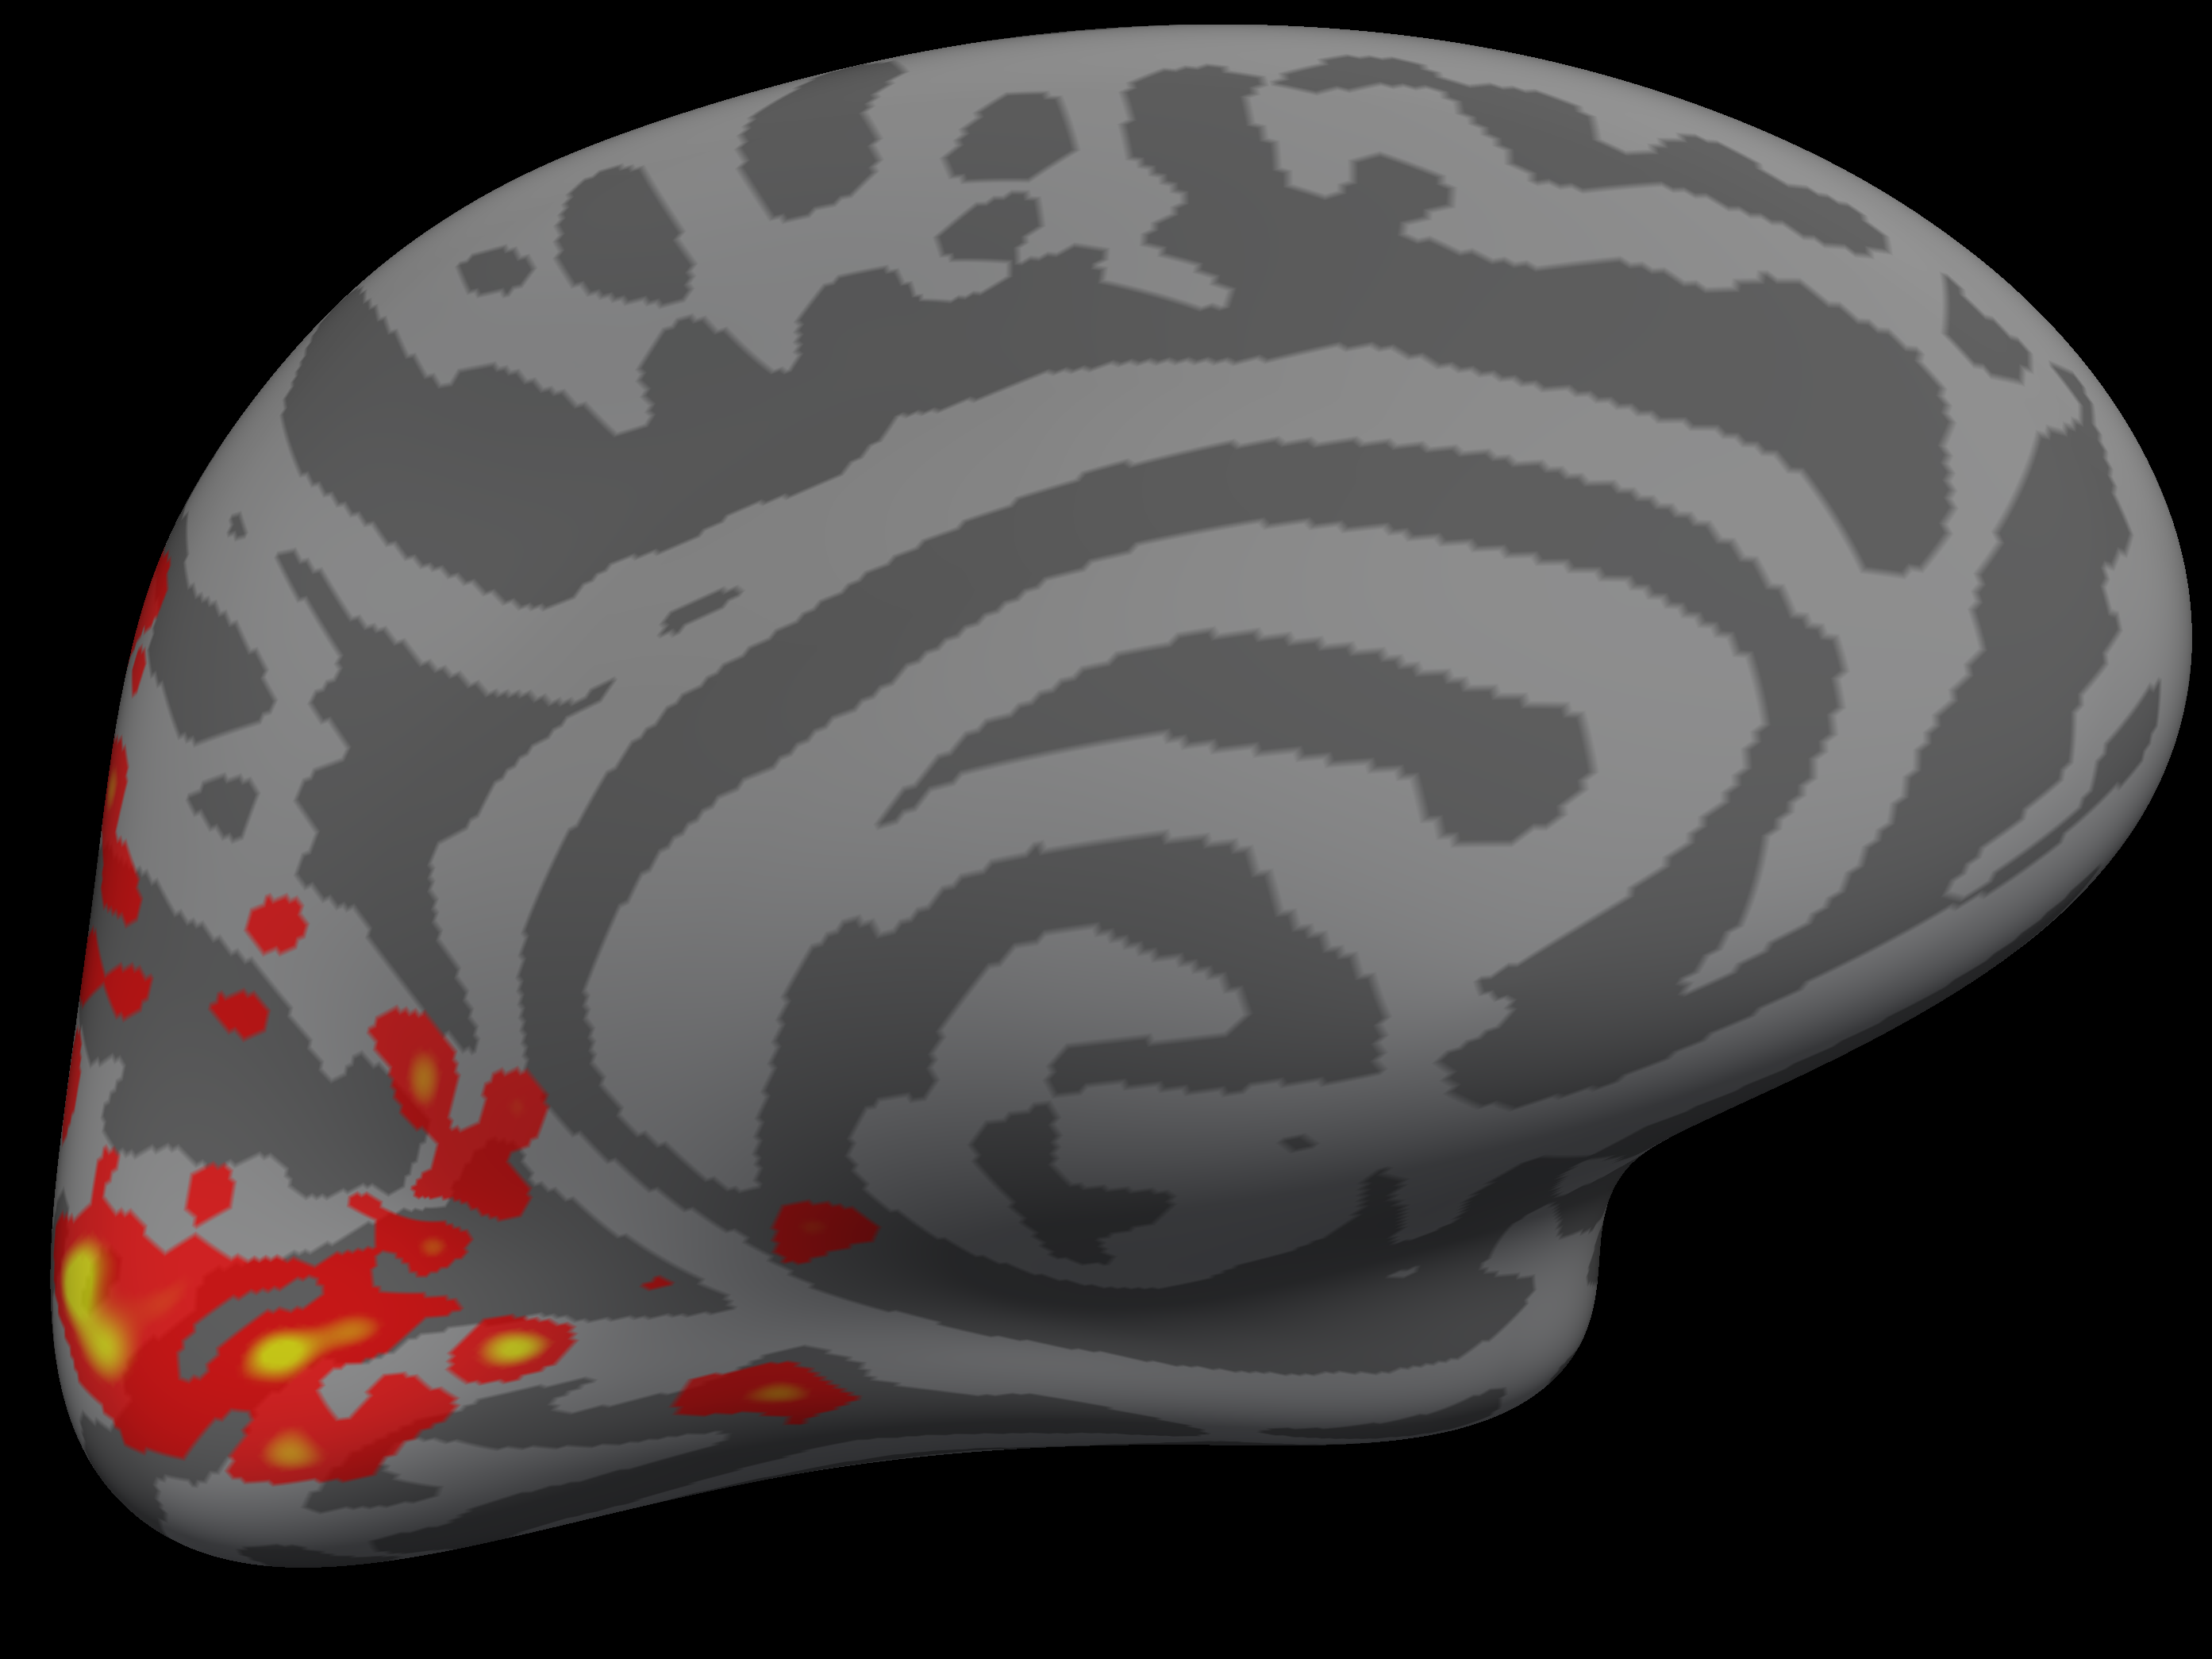
\includegraphics[width=\textwidth]{figures/lh-medial-smax-average}
\caption{}
\label{fig:lh-medial-smax-average}
\end{subfigure}
\begin{subfigure}{0.4\textwidth}
\centering
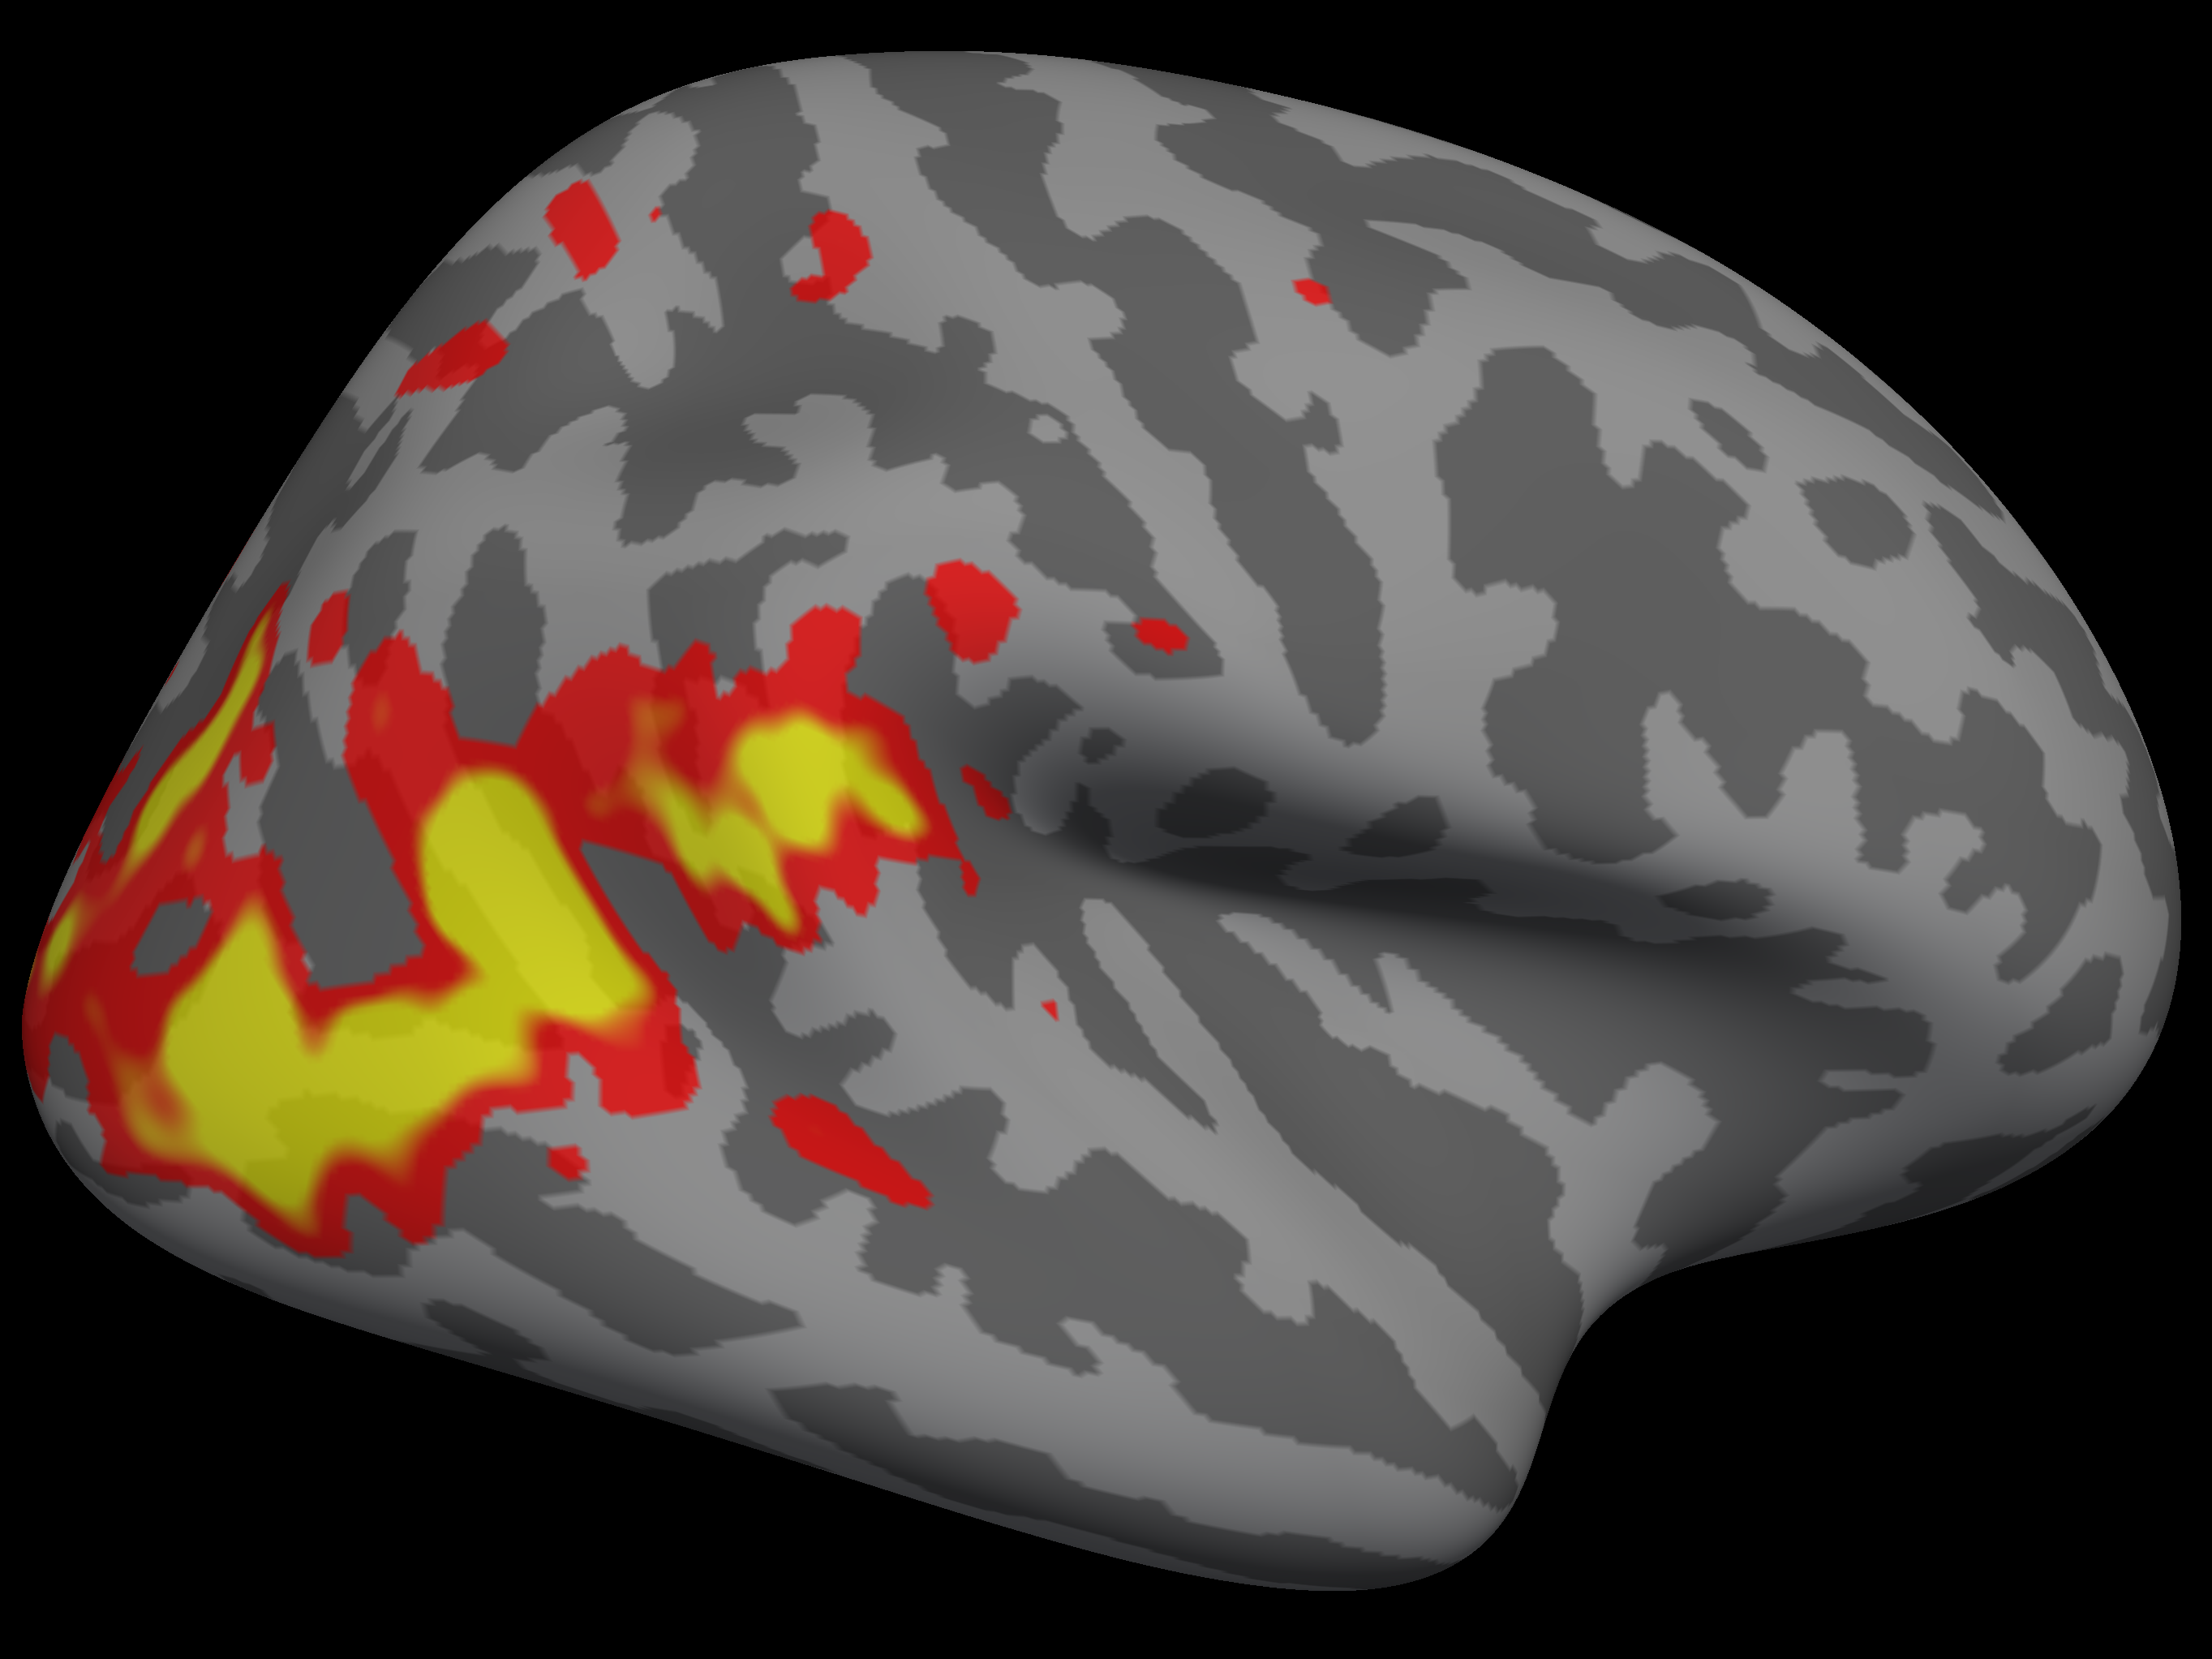
\includegraphics[width=\textwidth]{figures/rh-lateral-smax-average}
\caption{}
\label{fig:rh-lateral-smax-average}
\end{subfigure}
\begin{subfigure}{0.4\textwidth}
\centering
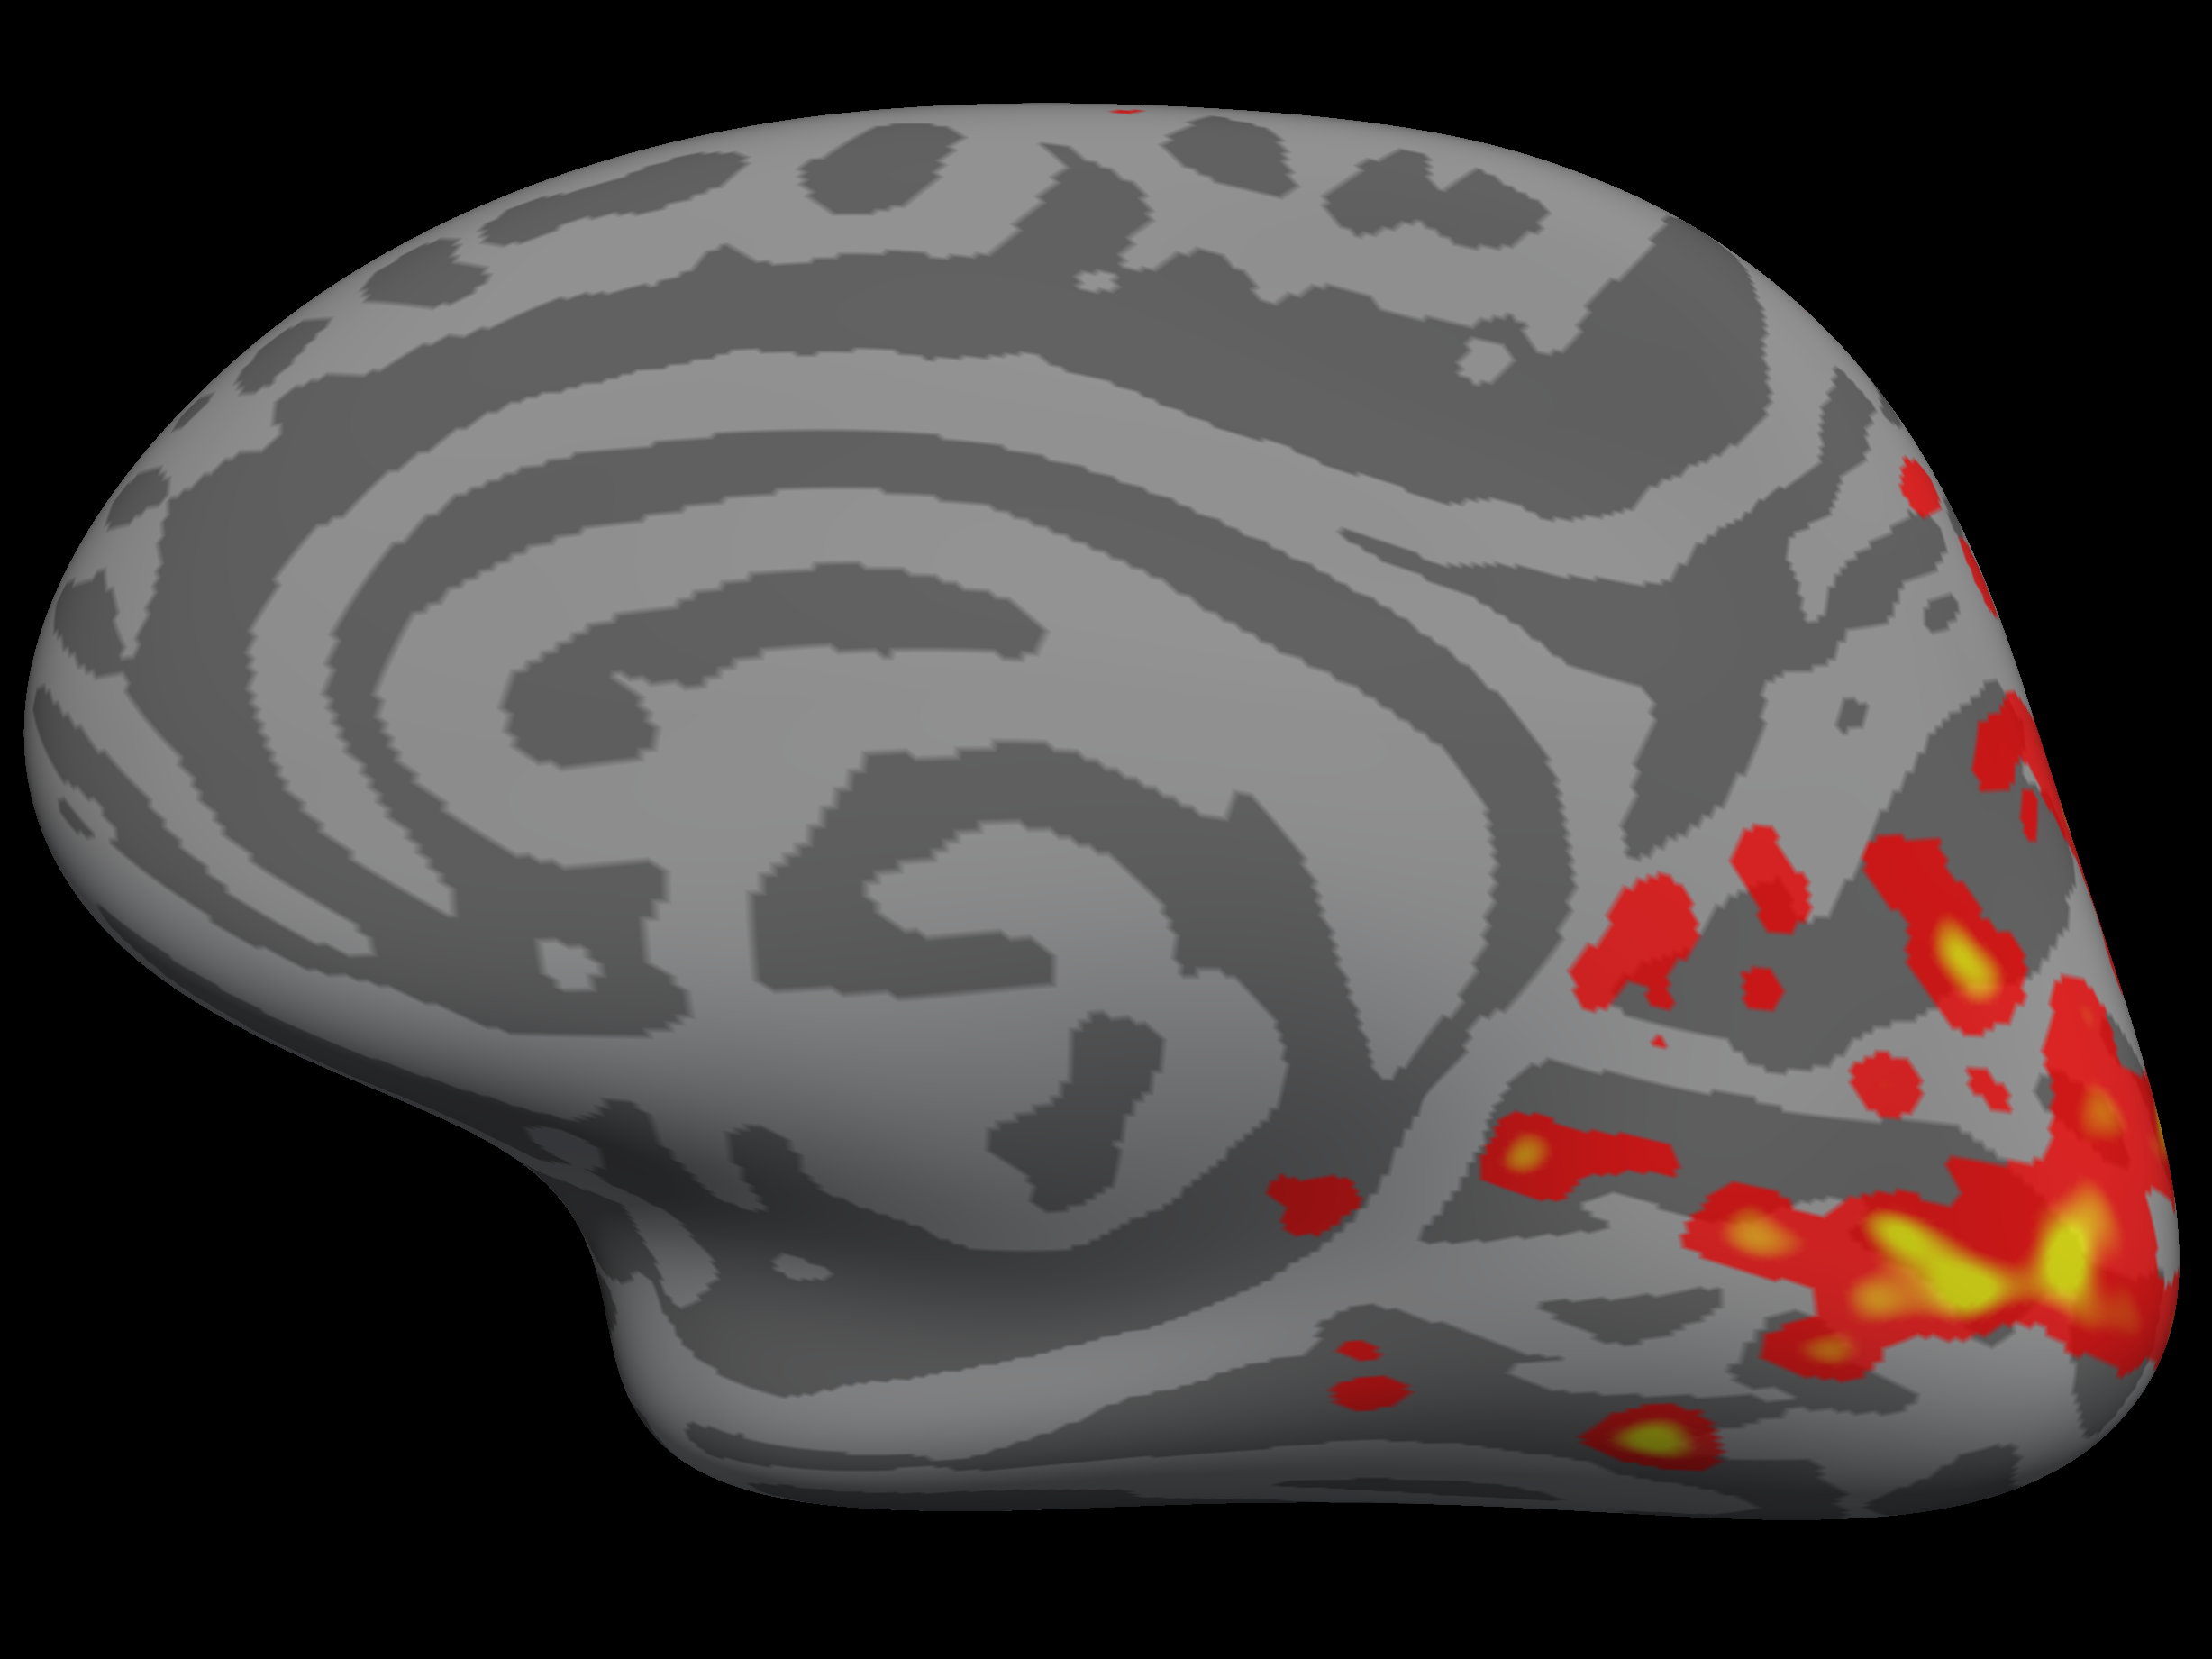
\includegraphics[width=\textwidth]{figures/rh-medial-smax-average}
\caption{}
\label{fig:rh-medial-smax-average}
\end{subfigure}
\caption{The sensitivity analysis averaged across all subjects.
Brighter regions indicate voxels that were important for successful discrimination by the machine-learning algorithms.}
\label{fig:preliminary-data-sensitivity}
\end{figure}
It is unclear whether the classifiers were measuring purely low level visual features to make their predictions or if higher-level object recognition circuits were involved.
Our new experiment will allow us to better understand the potential and limitations of applying machine learning techniques to this problem.

\section{Research Design}
We will be using an MRI machine to collect functional data from six subjects while they view a visual stimulus containing images of faces on a computer monitor and perform a simple visual task.
This data will then be preprocessed and analyzed by baseline machine learning algorithms in order to determine the resolvability of the perception of multiple objects.
Finally, we will experiment with more complex machine learning algorithms in order to improve the resolution of this measurement.
Due to the complexity of our experiment, we have divided our research plan into four distinct and relatively independent sections: fMRI, stimulus, preprocessing, and analysis.

\subsection{fMRI}
Data will be collected from the subjects using a Sieman's Skyra scanner with the product 32-channel head coil.
Functional data will be collected using the SENSE EPI product sequence with 2 millimeter cubic voxels, 50 slices, and a TR of 2.5 seconds.
The slice prescription will be oriented along the axis formed between the anterior and posterior commissures.
Before and after functional data collection, we will also record inplane T1-weighted anatomical images using the MP RAGE product sequence.
In a separate session, we will collect high resolution T1-weighted anatomical images also using the MP RAGE product sequence with 0.7 millimeter cubic voxels.

\subsection{Stimulus}
While functional data is being collected, the subjects will view a stimulus on a computer monitor and perform a simple task.
The stimulus employs a classic block presentation design where images are presented for 15 seconds followed by 15 seconds of an empty screen.
During each presentation period, images of faces and places are presented in a two by three grid.
An example frame is presented in figure \ref{fig:stimulus-frame}.
\begin{figure}
\centering
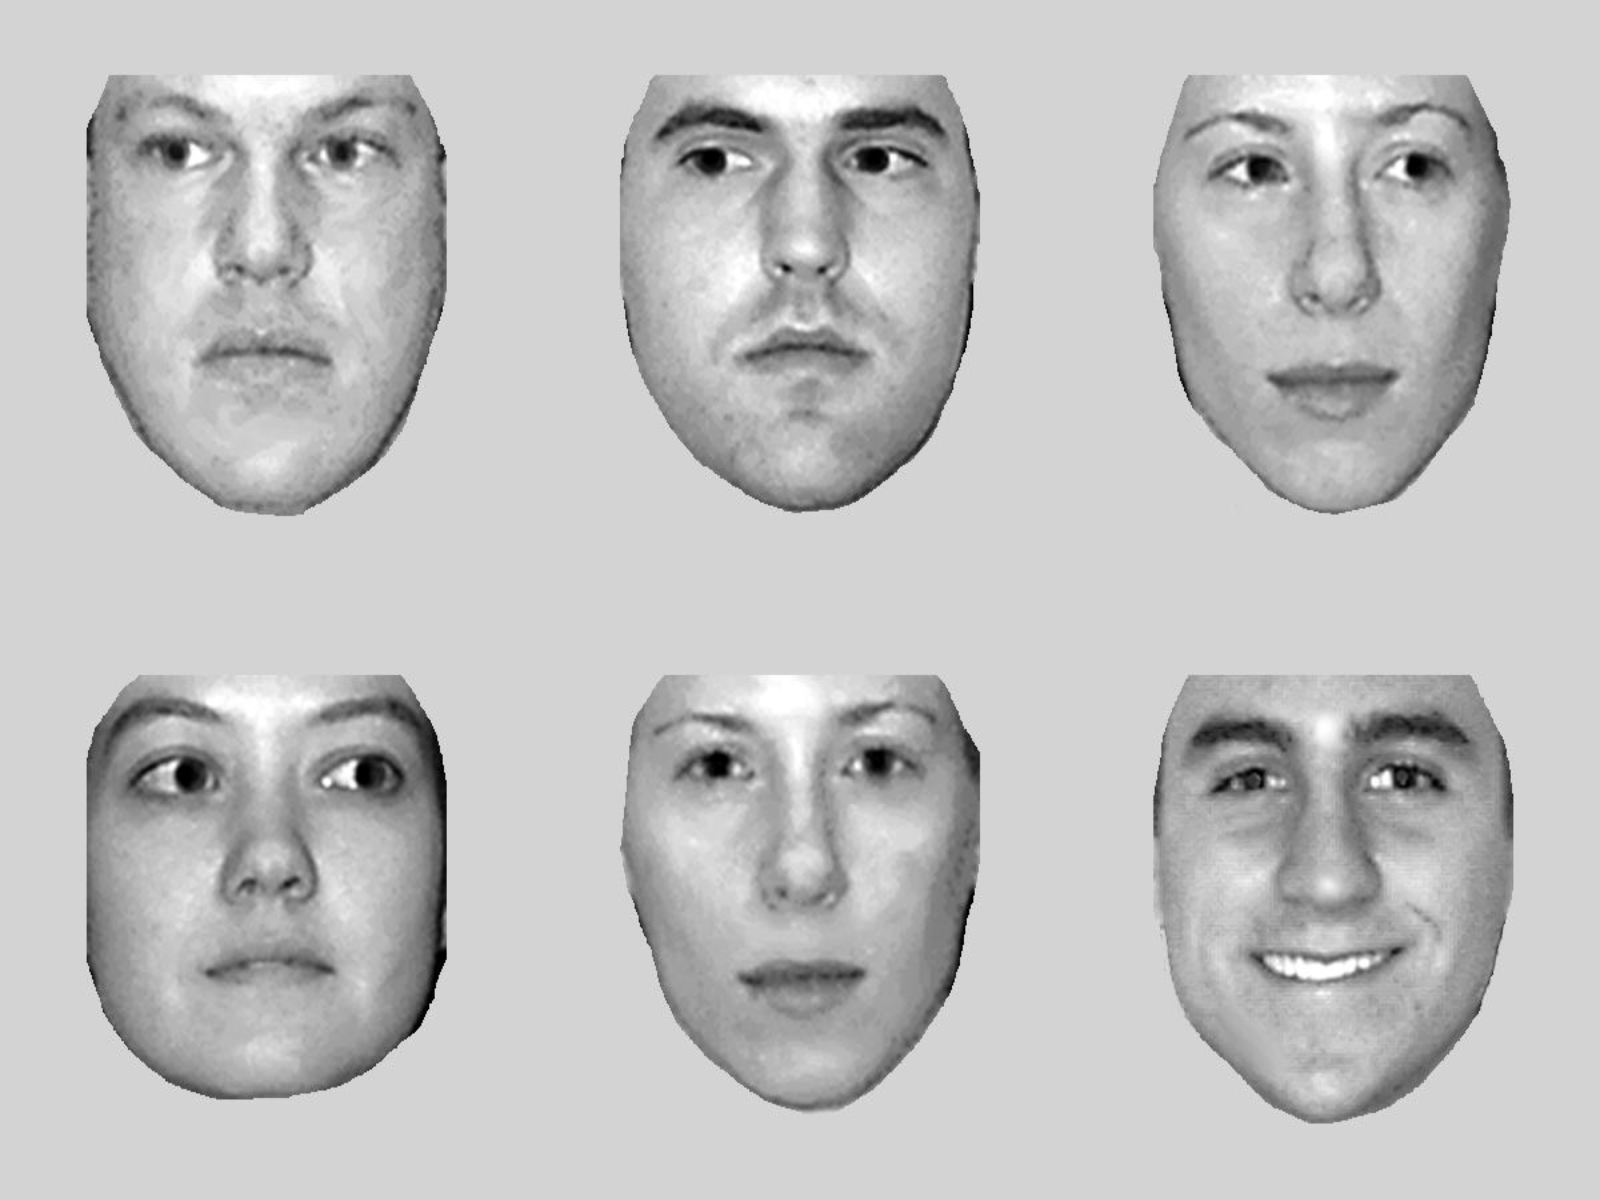
\includegraphics[width=0.5\textwidth]{figures/stimulus-frame}
\caption{An example frame from the stimulus to be used in our experiment.
This frame depicts an example when six faces are present, but the number and location of the faces can vary randomly from one to six.
Notice that the third image in the first row and the second image in the second row are different images of the same person.
Detecting the presence of different images of the same person or place in a single presentation is the task that the subjects will be performing.}
\label{fig:stimulus-frame}
\end{figure}
We are using the same face and place images used in \cite{Haxby2001}.
The images have had their contrasts normalized and have been closely cropped in order to limit confounding factors.
The database contains four images of six different people for a total of twenty-four face images.
Similarly, the database contains four images of six different locations for a total of twenty-four location images.
Some combination of one to six faces and zero to five places will appear during the image presentation.
To the subject, the presentation will be apparently random but the presentation order is controlled so that two examples for all six possible face counts will be present.
As a result, there will also be two examples for all six possible place counts in each run.
We plan to record two sessions for each subject and six runs during each session.
This will give us plenty of data with which to train our machine learning algorithms.

During this presentation procedure, the subjects will perform a simple task in order to properly direct their attentional resources.
The task will be to indicate whether two images of the same face or place appear during a single presentation.
To be specific, the exact same image will never appear in the same presentation but as previously discussed there are four different images of each face and place in the database.
This will ensure that the subjects carefully study each face and place during every presentation.
It is important that the task not employ memory between presentations as previous experiments \cite{Lewis-Peacock2012} have shown that differentiating between a subject viewing an image and a subject remembering an image can be difficult.

\subsection{Preprocessing}
We will perform standard inter- and intra-run motion compensation and slice timing correction \cite{Nestares2000}.
We will then concatenate each run to form a single time series for each session.
In order to correct for the time delay introduced by the hemodynamic response in the brain we will perform Wiener-filter deconvolution.
Wiener-filter deconvolution optimally deconvoles a signal using a known convolution kernel, in our case the hemodynamic response function, and a measure of the spectral signal to noise ratio (SNR) of the time series.
This SNR measurement is impractical if not impossible to make in fMRI due to the complex structure of the noise.
Therefore, we will manually adjust this value until the deconvolved signal has its phase properly adjusted without overly amplifying the noise.
This number will vary from run to run depending on the state of the scanner as well as the subject.

Before applying our machine learning algorithms to the data we will need to reduce the dimensionality.
Previous experiments \cite{Pereira2009} as well as our own have shown that an event related metric can be used to select useful voxels for training.
Performing this procedure will drastically reduce the input dimensionality of our problem from the total number of voxels ($\sim$500,000) to several thousand voxels.
We employ a procedure that we call harmonic analysis where we rank each voxel by the percent of the voxel's power spectrum contained in the stimulus' presentation frequency and its harmonics.
In this way, we select all voxels which covary in any way with respect to the stimulus.

\subsection{Analysis}
To determine the resolvability of the dimension of perceived object count we will estimate the performance of machine learning classifiers at predicting the presented number of faces in the stimulus.
Each frame in the time series will be labeled according to the number of faces presented to the subject at the time of image acquisition.
These labeled examples are presented to the machine learning algorithms in order to train them.
The trained algorithms are then tested by guessing the correct label of previously unpresented examples.
The performance of a machine learning algorithm on the dataset is defined to be the probability that a previously unpresented example will be labeled correctly.
This measure of performance can only be estimated due to the finite number of examples.

In order to minimize the bias of our estimate of performance, we will test our machine learning algorithms using a cross-validation approach \cite{Kohavi1995}.
First, the entire dataset is split into $N$ partitions or folds.
Each machine learning algorithm is trained on every example in $N-1$ folds and performance is tested on the remaining fold.
This is repeated for all $N$ folds and the performance from each fold is averaged to obtain the final estimate of performance for each algorithm.
Researchers have noted that temporal correlation between adjacent frames can lead to overly optimistic estimates of performance if adjacent frames are present in the training and test sets \cite{Pereira2009}.
Therefore, the folds will be selected such that a minimum average temporal distance is maintained between all of the folds.
Additionally, we will ensure that number of examples of each face count is equally represented in all of the folds.
This is knows as stratified cross-fold validation \cite{Kohavi1995} and it leads to a less biased estimate of classifier performance.

With a method for accurately estimating the performance of machine learning classifiers on our dataset we can compare and develop better classification techniques.
Initially, we will estimate the performance of the classic linear SVMs and feed-forward neural networks.
Previous work and our own preliminary results indicate that these basic approaches work very well and they will serve is a good baseline for comparing other algorithms.
We will then analyze more complex recurrent neural networks, such as Restricted Boltzmann Machines, and non-linear support vector machines in order to discover improved classification techniques.
Improved classification techniques directly translate to improved resolution along the dimension of perceived object count and will likely lead to improved resolution in other dimensions as well.
New measureable dimensions and improved resolution along those dimensions in turn will lead to new insightful behavioral and cognitive experiments.

\bibliography{bib}

\end{document}
